\documentclass{article}[18pt]
\ProvidesPackage{format}
%Page setup
\usepackage[utf8]{inputenc}
\usepackage[margin=0.7in]{geometry}
\usepackage{parselines} 
\usepackage[english]{babel}
\usepackage{fancyhdr}
\usepackage{titlesec}
\hyphenpenalty=10000

\pagestyle{fancy}
\fancyhf{}
\rhead{Sam Robbins}
\rfoot{Page \thepage}

%Characters
\usepackage{amsmath}
\usepackage{amssymb}
\usepackage{gensymb}
\newcommand{\R}{\mathbb{R}}

%Diagrams
\usepackage{pgfplots}
\usepackage{graphicx}
\usepackage{tabularx}
\usepackage{relsize}
\pgfplotsset{width=10cm,compat=1.9}
\usepackage{float}

%Length Setting
\titlespacing\section{0pt}{14pt plus 4pt minus 2pt}{0pt plus 2pt minus 2pt}
\newlength\tindent
\setlength{\tindent}{\parindent}
\setlength{\parindent}{0pt}
\renewcommand{\indent}{\hspace*{\tindent}}

%Programming Font
\usepackage{courier}
\usepackage{listings}
\usepackage{pxfonts}

%Lists
\usepackage{enumerate}
\usepackage{enumitem}

% Networks Macro
\usepackage{tikz}


% Commands for files converted using pandoc
\providecommand{\tightlist}{%
	\setlength{\itemsep}{0pt}\setlength{\parskip}{0pt}}
\usepackage{hyperref}

% Get nice commands for floor and ceil
\usepackage{mathtools}
\DeclarePairedDelimiter{\ceil}{\lceil}{\rceil}
\DeclarePairedDelimiter{\floor}{\lfloor}{\rfloor}

% Allow itemize to go up to 20 levels deep (just change the number if you need more you madman)
\usepackage{enumitem}
\setlistdepth{20}
\renewlist{itemize}{itemize}{20}

% initially, use dots for all levels
\setlist[itemize]{label=$\cdot$}

% customize the first 3 levels
\setlist[itemize,1]{label=\textbullet}
\setlist[itemize,2]{label=--}
\setlist[itemize,3]{label=*}

% Definition and Important Stuff
% Important stuff
\usepackage[framemethod=TikZ]{mdframed}

\newcounter{theo}[section]\setcounter{theo}{0}
\renewcommand{\thetheo}{\arabic{section}.\arabic{theo}}
\newenvironment{important}[1][]{%
	\refstepcounter{theo}%
	\ifstrempty{#1}%
	{\mdfsetup{%
			frametitle={%
				\tikz[baseline=(current bounding box.east),outer sep=0pt]
				\node[anchor=east,rectangle,fill=red!50]
				{\strut Important};}}
	}%
	{\mdfsetup{%
			frametitle={%
				\tikz[baseline=(current bounding box.east),outer sep=0pt]
				\node[anchor=east,rectangle,fill=red!50]
				{\strut Important:~#1};}}%
	}%
	\mdfsetup{innertopmargin=10pt,linecolor=red!50,%
		linewidth=2pt,topline=true,%
		frametitleaboveskip=\dimexpr-\ht\strutbox\relax
	}
	\begin{mdframed}[]\relax%
		\centering
		}{\end{mdframed}}



\newcounter{lem}[section]\setcounter{lem}{0}
\renewcommand{\thelem}{\arabic{section}.\arabic{lem}}
\newenvironment{defin}[1][]{%
	\refstepcounter{lem}%
	\ifstrempty{#1}%
	{\mdfsetup{%
			frametitle={%
				\tikz[baseline=(current bounding box.east),outer sep=0pt]
				\node[anchor=east,rectangle,fill=blue!20]
				{\strut Definition};}}
	}%
	{\mdfsetup{%
			frametitle={%
				\tikz[baseline=(current bounding box.east),outer sep=0pt]
				\node[anchor=east,rectangle,fill=blue!20]
				{\strut Definition:~#1};}}%
	}%
	\mdfsetup{innertopmargin=10pt,linecolor=blue!20,%
		linewidth=2pt,topline=true,%
		frametitleaboveskip=\dimexpr-\ht\strutbox\relax
	}
	\begin{mdframed}[]\relax%
		\centering
		}{\end{mdframed}}
\lhead{Software Engineering - Software Design}


\begin{document}
\begin{center}
\underline{\huge The major forms of architectural style}
\end{center}
\section{Call and return}
Characterised by:
\begin{itemize}
	\item Order of computation (sequencing of control)
	\item Only a single thread of control (no concurrency)
	\item Structures organised around computational tasks
\end{itemize}
Type of reasoning:
\begin{itemize}
	\item Hierarchical, organised around control being passed from "higher" to "lower" items
	\item Task performed by a set of sub-tasks
	\item Explicit control linkages between the subtasks and the algorithm of the program to determine calling order
\end{itemize}
\subsection{Example 1}
Main program/sub-programs:
\begin{itemize}
	\item Components are subprograms
	\item Connectors are the invocation links (including parameters)
\end{itemize}
This is the form that is embodied in most non-OO imperative programming languages
\begin{center}
	\includegraphics[scale=0.7]{"Call and Return"}
\end{center}
\subsection{Example 2}
Classical objects - here the methods are part of the objects:
\begin{itemize}
	\item Components are both the objects and also their methods/data
	\item Connectors are the method calls and parameters
\end{itemize}
Supported by object-based and object-oriented programming languages. May use run-time bindings
\begin{center}
	\includegraphics[scale=0.7]{"Call and Return1"}
\end{center}
\section{Interacting Processes}
Characterised by:
\begin{itemize}
	\item Communication patterns among independent, usually concurrent, processes
	\item Independent elements can be objects, lightweight processes, services etc
	\item Context is more complex as emphasis is upon "interaction"
\end{itemize}
Type of reasoning
\begin{itemize}
	\item Non-deterministic - scheduling of system elements is performed by separate, independent computers
	\item Design based around these independent actions and needs to specifically address any requirements that impose the need for particular sequences or interactions
\end{itemize}
\subsection{Communicating processes}
Based around a network of processes running on different machines and linked via Remote Procedure Calls (RPC)
\begin{itemize}
	\item Components are the processes
	\item Connectors are the message protocols via RPCs
\end{itemize}
Binding time can be at each construction or when the system is started. Each system runs in its own address space - no direct access to shared data
\begin{center}
	\includegraphics[scale=0.7]{"Communicating Processes"}
\end{center}
\subsection{Lightweight processes (threads)}
A thread is a block of code that can be executed independently of other threads within the program
\begin{itemize}
	\item Components are the threads
	\item Connectors are provided largely by using shared data
\end{itemize}
Because threads are part of a single process, they have a shared data space, needing care with synchronisation of access
\begin{center}
	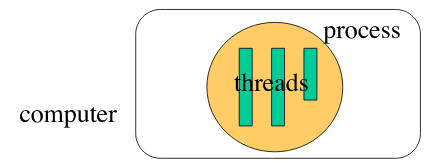
\includegraphics[scale=0.7]{Threads}
\end{center}
\section{Data-Centred Repository}
Characterised by:
\begin{itemize}
	\item A dominant central data store that is manipulated by independent communications
	\item Centred around the issues relating to data access 
	\item Data is at the focus
\end{itemize}
Type of reasoning:
\begin{itemize}
	\item Can depend on the form of the system
	\item For databases it is the ACID properties
	\item Includes modern compilers
\end{itemize}
\subsection{Transactional Database}
The classical idea of the data-centred repository
\begin{itemize}
	\item Components - Memory and computations within the database
	\item Connectors - Transaction streams (queries)
\end{itemize}
Style is not concerned with the internal form of the database, only with its role
\begin{center}
	\includegraphics[scale=0.7]{"Transactional Database"}
\end{center}
\subsection{Client-Server}
A "distributed" form using a "thin" client process to interact with the end-users. While the server often incorporates a database, this is not a necessity
\begin{itemize}
	\item Components - Data managers and computations
	\item Connectors - Transaction operations with history
\end{itemize}
The history element is important, systems that lack this are sometimes termed "naive client-server" forms
\section{Data-Sharing}
Characterised by:
\begin{itemize}
	\item Direct sharing of data between the components
	\item Data may be distributed between many elements, but these share a common form of "representation" for using and sharing this data
\end{itemize}
Type of reasoning:
\begin{itemize}
	\item Based upon the data representation itself and ensuring that this is common to all elements
	\item Describes both programs, but also documents
\end{itemize}
\subsection{Hypertext}
This is a "document" form rather than a program form, but still an important architectural style since it affects the way that programs are structured in order to use it
\begin{itemize}
	\item Components - Documents in HTML format
	\item Connectors - Hyperlinks and internal anchors
\end{itemize}
Websites can incorporate both static pages and also pages that are generated dynamically, so this example is quite an important one.
\section{Mixed styles}
An example of a mixed style is a compiler, it started out as pipe and filter, but are now usually more of a data-centred repository.
\section{Shaw and Clement's classification}
\begin{itemize}
	\item Context is elaborated by being sub-divided into three aspects (control, data and control/data interaction) which are further sub-divided
	\item In addition, they consider the form of reasoning that might be used with a particular architectural style
\end{itemize}
Control issues are classified in terms of:
\begin{itemize}
	\item Topology (geometric form)
	\item Synchronicity (interdependence of actions and states)
	\item Binding time (when is the identify of a partner established)
\end{itemize}
Data issues are classified using:
\begin{itemize}
	\item Topology - same concept as for control
	\item Continuity - e.g. continuous flow of data or sporadic flow
	\item Mode - whether data is copied, shared etc
	\item Binding time (as for control)
\end{itemize}
Control/data interaction captures some further relationships, and is classified in terms of
\begin{itemize}
	\item Share (are control and data flow topologies isomorphic?)
	\item Directionality (if the shapes are the same, does control flow in the same direction as data, or in the opposite direction)
\end{itemize}
\section{Architectural Mismatch}
\begin{definition}[Architectural Mismatch]
Mismatched assumptions a reusable part makes about the system it is to be a part of
\end{definition}
Basic cause was in the detail (of components, connectors and context). Each element had a slightly different model of how control and event passing was organised, reinforcing the point that all of the different aspects of architectural style are relevant
\section{Security}
\begin{itemize}
	\item The way this is handled will depend on architectural style
	\item Each style will exhibit its own vulnerabilities
	\begin{itemize}
		\item How does a component check or confirm that is it connected to a valid component
		\item How might it be attacked
		\item How easily can we achieve "information hiding" within a particular architectural style
	\end{itemize}
	\item Increasingly, this adds a new dimension to those that the designer has to think of
\end{itemize}
\section{Choosing a style}
Some guidelines on choice of style, where this is not already determined by other factors:
\begin{itemize}
	\item For strongly sequential tasks: batch sequential or pipe-and-filter
	\item For tasks which involve transformation on continuous streams of data, use pipe-and-filter
	\item If a central issue in your system is understanding the data used in the application, consider a repository style
	\item For flexibility, loose coupling between tasks and reactive tasks, consider interacting processes
\end{itemize}





\end{document}